\documentclass{article}
\usepackage{geometry}
 \geometry{
 a4paper,
 total={170mm,270mm},
 left=20mm,
 top=10mm,
 }
\usepackage{graphicx}
\usepackage{float}
\usepackage{enumitem}
\usepackage{caption}
\usepackage{amsmath}
\newcommand*{\addheight}[2][.5ex]{%
  \raisebox{0pt}[\dimexpr\height+(#1)\relax]{#2}%
}
\title{\textbf{Chaotic Dynamics - CSCI 5446} \\
Problem Set 5}
\author{Santhanakrishnan Ramani}
\begin{document}
\maketitle

\section*{Problem 2}
\begin{enumerate}[label=(\alph*)]
\item 
The Figure \ref{fig:prob2a} represents the projection on the x-z plane of the plot of a chaotic attractor in the Lorenz System with a = 16, r = 45, b = 4, starting from the initial condition (x,y,z) = (-13, -12, 52).\par\medskip
\begin{minipage}{\linewidth}
{
\centering 
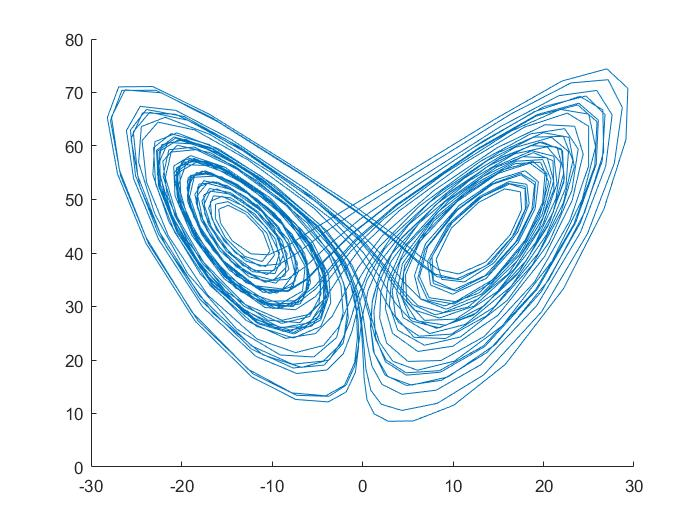
\includegraphics[scale=0.4]{images/prob2a.jpg}
\captionof{figure}{Lorenz system}
\label{fig:prob2a}
}
\par\medskip
\end{minipage}

\item
The Figure \ref{fig:prob2b} represents the overlay of the results of adaptive integrator from prob 2(a) and nonadaptive integrator to plot a trajectory for the same initial condition in prob 2(a) using a timestep of 0.001.
\begin{minipage}{\linewidth}
{
\centering 
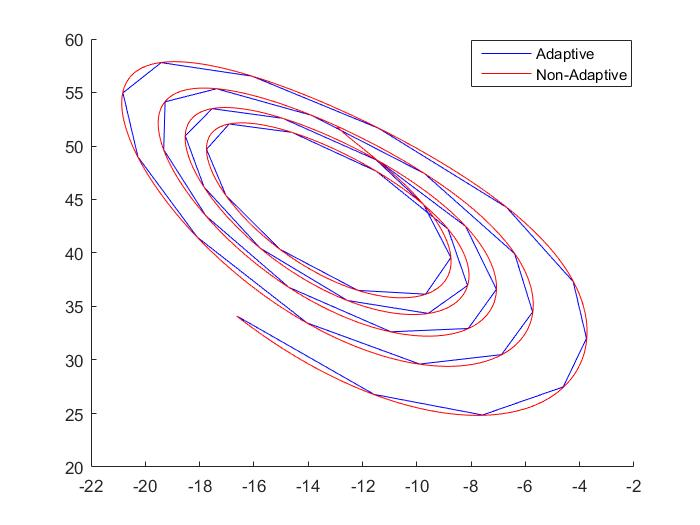
\includegraphics[scale=0.4]{images/prob2b.jpg}
\captionof{figure}{Adaptive vs Non-Adaptive RK4}
\label{fig:prob2b}
}
\par\medskip
Yes, the two solutions agree, the adaptive reaches the point quicker whereas the non-adaptive takes a bit more steps. The points produced by adaptive solver aren't evenly spaced in time.
\end{minipage}
\newpage
\item
On keeping a \& b values fixed and increasing the value of r,
\textbf{$0 < r < 1$}, the system converges to the origin, a stable fixed point.
\textbf{$13.5 < r < 14$}, the system converges to a stable fixed point on the left of the origin initially and shifts to the one on the right.
\textbf{$23 < r < 30$}, the system continues to converge to stable fixed point, but suddenly starts to get repelled from the fixed point and displays chaotic behavior.

\end{enumerate}

\section*{Problem 3}
The Figure \ref{fig:prob3} represents the projection on the x-z plane of the plot of the chaotic attractor in the Rossler system with a = .398, b = 2, c = 4.\par\medskip
\begin{minipage}{\linewidth}
{
\centering 
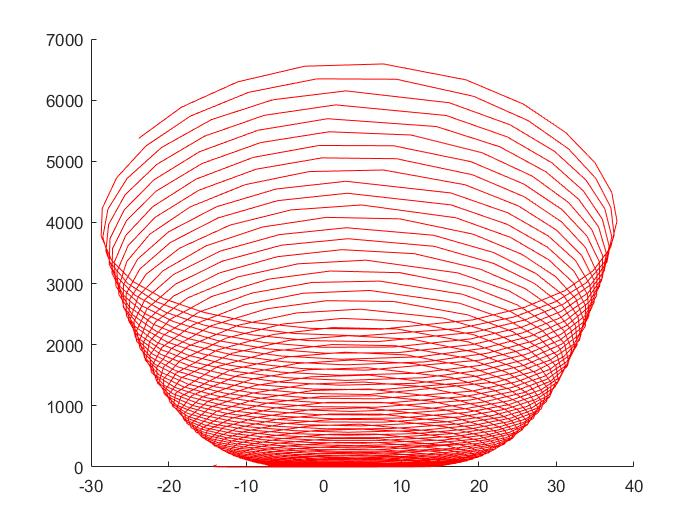
\includegraphics[scale=0.4]{images/prob3.jpg}
\captionof{figure}{Rossler System}
\label{fig:prob3}
}
\end{minipage}

\section*{Problem 4}
\begin{table}[H]
\centering
\begin{tabular}{|c|c|}
	\hline
	\addheight{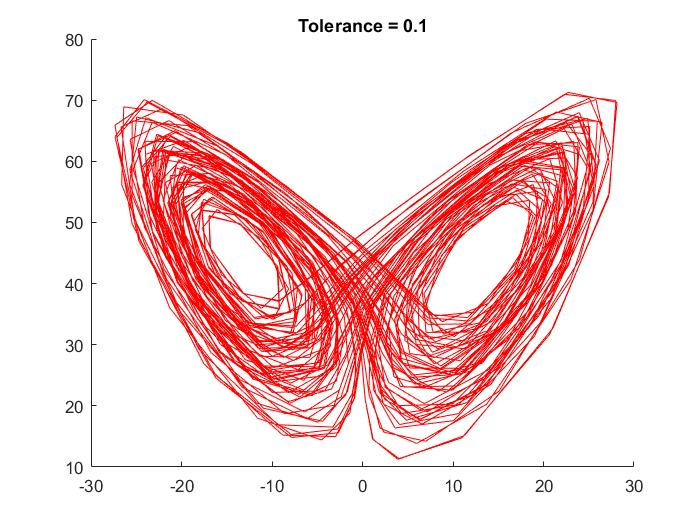
\includegraphics[width=80mm]{images/prob4a.jpg}} &
    \addheight{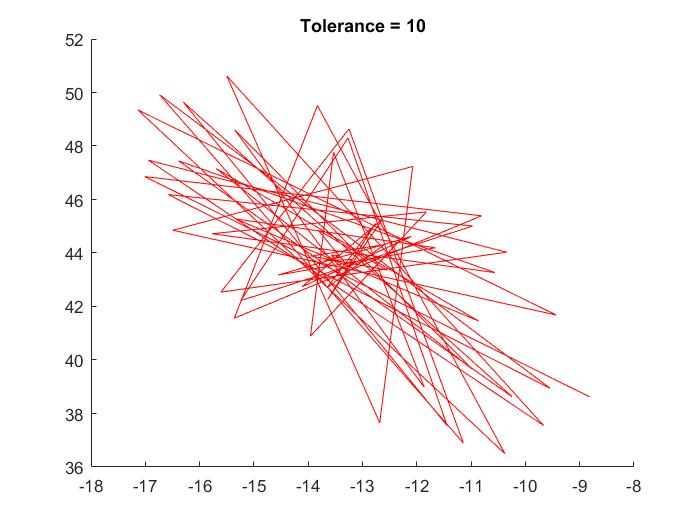
\includegraphics[width=80mm]{images/prob4b.jpg}} \\
    \hline
\end{tabular}
\end{table}

The breakdown in dynamics of the Lorenz System is clearly evident from the above diagrams as the value of error bound is increased, this is very much similar to the result of timeStep exploration in the previous problem set. One difference I felt was the system initially converged and then diverged on increasing timeStep, whereas in this case, on increasing the error bound for the conditions given in prob 2, the systems goes from diverging to converging.
\end{document}
